%package list
\documentclass{article}
\usepackage[top=3cm, bottom=3cm, outer=3cm, inner=3cm]{geometry}
\usepackage{graphicx}
\usepackage{url}
%\usepackage{cite}
\usepackage{hyperref}
\usepackage{array}
\usepackage{multicol}
\newcolumntype{x}[1]{>{\centering\arraybackslash\hspace{0pt}}p{#1}}
\usepackage{natbib}
\usepackage{pdfpages}
\usepackage{multirow}
\usepackage{float}
\usepackage[normalem]{ulem}
\useunder{\uline}{\ul}{}

\usepackage{listings}
\usepackage{xcolor}
\usepackage{algorithm,algorithmic}

% For Logic syntax
\usepackage{fitch}
\usepackage{bussproofs}
\renewcommand{\fCenter}{\vdash}

\definecolor{codegreen}{rgb}{0,0.6,0}
\definecolor{codegray}{rgb}{0.5,0.5,0.5}
\definecolor{codepurple}{rgb}{0.58,0,0.82}
\definecolor{backcolour}{rgb}{0.95,0.95,0.92}

\lstdefinestyle{style_code}{
    backgroundcolor=\color{backcolour},   
    commentstyle=\color{codegreen},
    keywordstyle=\color{magenta},
    numberstyle=\tiny\color{codegray},
    stringstyle=\color{codepurple},
    basicstyle=\ttfamily\footnotesize,
    breakatwhitespace=false,         
    breaklines=true,                 
    captionpos=b,                    
    keepspaces=true,                 
    numbers=left,                    
    numbersep=5pt,                  
    showspaces=false,                
    showstringspaces=false,
    showtabs=false,                  
    tabsize=2
}

\lstset{style=style_code}



%%%%%%%%%%%%%%%%%%%%%%%%%%%%%%%%%%%%%%%%%%%%%%%%%%%%%%%%%%%%%%%%%%%%%%%%%%%%
%%%%%%%%%%%%%%%%%%%%%%%%%%%%%%%%%%%%%%%%%%%%%%%%%%%%%%%%%%%%%%%%%%%%%%%%%%%%
\newcommand{\csemail}{mquispecr@unsa.edu.pe}
\newcommand{\csdocente}{Marcela Quispe Cruz}
\newcommand{\cscurso}{Teoría de la Computación}
\newcommand{\csuniversidad}{Universidad Nacional de San Agustín}
\newcommand{\csescuela}{Maestría en Ciencia de la Computación}
\newcommand{\cspracnr}{01}
\newcommand{\cstema}{Lógica Proposicional}
%%%%%%%%%%%%%%%%%%%%%%%%%%%%%%%%%%%%%%%%%%%%%%%%%%%%%%%%%%%%%%%%%%%%%%%%%%%%
%%%%%%%%%%%%%%%%%%%%%%%%%%%%%%%%%%%%%%%%%%%%%%%%%%%%%%%%%%%%%%%%%%%%%%%%%%%%


\usepackage[english,spanish]{babel}
\usepackage[utf8]{inputenc}
\AtBeginDocument{\selectlanguage{spanish}}
\renewcommand{\figurename}{Figura}
\renewcommand{\refname}{Referencias}
\renewcommand{\tablename}{Tabla} %esto no funciona cuando se usa babel
\AtBeginDocument{%
	\renewcommand\tablename{Tabla}
}

\usepackage{fancyhdr}
\pagestyle{fancy}
\fancyhf{}
\setlength{\headheight}{30pt}
\renewcommand{\headrulewidth}{1pt}
\renewcommand{\footrulewidth}{1pt}
\fancyhead[L]{\raisebox{-0.2\height}{
\includegraphics[width=3cm]{img/logo_unsa}}}
\fancyhead[C]{}
\fancyhead[R]{\fontsize{7}{7}\selectfont	\csuniversidad \\ \csescuela \\ \textbf{\cscurso} }
\fancyfoot[L]{Dra. Marcela Quispe Cruz}
\fancyfoot[C]{\cscurso}
\fancyfoot[R]{Página \thepage}







\begin{document}
	
	\vspace*{10px}
	
	\begin{center}	
		\fontsize{17}{17} \textbf{ Práctica \cspracnr}
	\end{center}
	%\centerline{\textbf{\underline{\Large Título: Informe de revisión del estado del arte}}}
	%\vspace*{0.5cm}
	

	\begin{table}[h]
		\begin{tabular}{|x{4.7cm}|x{4.8cm}|x{4.8cm}|}
			\hline 
			\textbf{DOCENTE} & \textbf{CARRERA}  & \textbf{CURSO}   \\
			\hline 
			\csdocente & \csescuela & \cscurso    \\
			\hline 
		\end{tabular}
	\end{table}	
	
	
	\begin{table}[h]
		\begin{tabular}{|x{4.7cm}|x{4.8cm}|x{4.8cm}|}
			\hline 
			\textbf{PRÁCTICA} & \textbf{TEMA}  & \textbf{DURACIÓN}   \\
			\hline 
			\cspracnr & \cstema & 3 horas   \\
			\hline 
		\end{tabular}
	\end{table}
	
	
	\section{Datos de los estudiantes}
	\begin{itemize}
		\item Grupo: 9
		\item Integrantes: 
		\begin{itemize}
			\item Abarca Murillo, Jhonatan Piero
			\item Apari Pinto, Christian Timoteo
			\item Suca Velando, Christian Anthony
			\item Vargas Zuni, Arturo
		\end{itemize}
		
	\end{itemize}
	

	
	\section{Ejercicios}\label{sec:ejercicios}
	\begin{enumerate}

		\item Existen dos cajas, A y B. Un aviso en la caja A dice ``El aviso en la caja B es falso y el oro está en la caja B". Un aviso en la caja B dice ``El aviso en la caja A es verdadero y el oro está en la caja B". Asumiendo que existe oro en una de las cajas, ¿cuál de ellas contiene oro? Justifique esa respuesta en términos lógicos.
		\\
		Declarando las variables:
		\begin{itemize}
		    \item p: Aviso en A es verdadero
		    \item q: Aviso en B es verdadero
		    \item r: El oro esta en A
		    \item s: El oro esta en B
		\end{itemize}
		\begin{enumerate}
		    \item \{El aviso en A \} si y solo si \{El aviso en la caja B es falso\} y \{el oro está en la caja B\}
    		    \[ p \Leftrightarrow (\neg q \land s) \]
		        
		    \item \{El aviso en B \} si y solo si \{El aviso en la caja A es verdadero\} y \{el oro está en la caja B\}
		        \[
		            q \Leftrightarrow (p \land s)
		        \]
		        
		    \item \{El oro esta en A \} o \{El oro esta en B \}
		         \[
		            r \lor s
		        \]
		\end{enumerate}
		
		La premisa quedaría de la siguiente manera
		
		        \begin{equation}
		            \{  p \Leftrightarrow (\neg q \land s) , q \Leftrightarrow (p \land s) ,  r \lor s \} \models r
		        \end{equation}
		        \begin{equation}
		            \{  p \Leftrightarrow (\neg q \land s) , q \Leftrightarrow (p \land s) ,  r \lor s \} \models s
		        \end{equation}
		
		Realizando el Tableaux en cada una de las premisas definidas para cada una tanto para $r$ y $s$, llegando solamente a concluir en $r$ (ver figura \ref{fig:1_1} ya que en $s$ no llega a ser válido. Concluyendo que \textbf{El oro esta en A}.
		
		\begin{figure}[H]
			\centering
			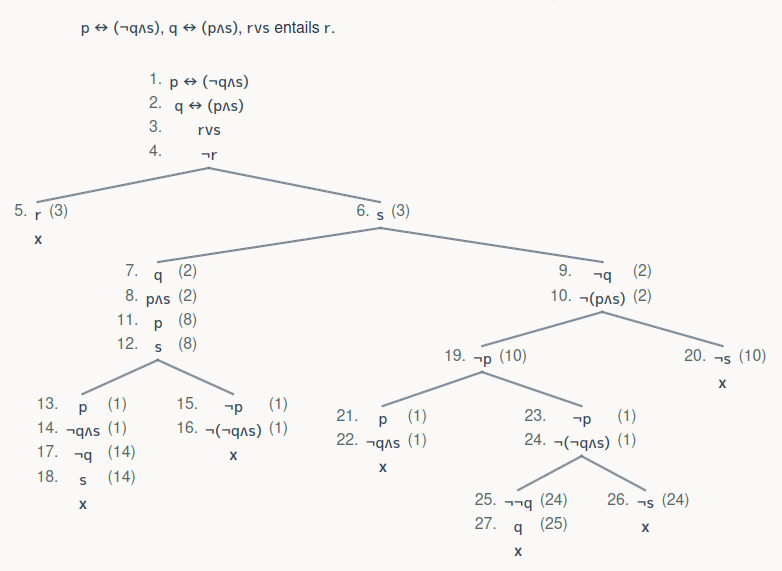
\includegraphics[scale=0.40]{img/1_1.png}
			\caption{ Demostración por Tableaux para $r$}
			\label{fig:1_1}
		\end{figure}
		
		\item Un crimen es cometido por una y solamente una persona y hay cuatro sospechosos: Paulo, Rodrigo, Enrique y Felipe. Interrogados ellos hacen las siguientes declaraciones:
		\begin{itemize}
		    \item \textbf{Felipe:} Rodrigo miente cuando dice que yo no soy inocente.
            \item \textbf{Paulo:} Rodrigo no es inocente.
            \item \textbf{Enrique:} Yo soy inocente.
            \item \textbf{Rodrigo:} Felipe no es inocente.
		\end{itemize}       
		
		Represente en lógica proposicional las sentencias arriba. Con base en estas sentencias lógicas, muestre que si el inspector usa Tableaux irá a concluir que si Enrique fuera culpable entonces solamente Felipe dice la verdad. Muestre el Tableaux que soporta la conclusión del inspector.
		
		
		

		Solución \\
		\begin{itemize}
		    \item f: Felipe dice la verdad
		    \item r: Rodrigo dice la verdad
		    \item e: Enrique dice la verdad
		    \item p: Paulo dice la verdad
		    \item a: Felipe es inocente
		    \item b: Rodrigo es inocente
		    \item c: Enrique es inocente
		    \item d: Paulo es inocente
		\end{itemize}
		
		Proposiciones \\
		\begin{equation}
		   \begin{aligned}
             \neg a  \to  ( b \land c \land d), \neg b  \to  ( a \land c \land d), \neg c  \to  ( b \land a \land d), \neg d  \to  ( b \land c \land a), \\f \Leftrightarrow  \neg r \land a,
            p \Leftrightarrow \neg b,e \Leftrightarrow c, r \Leftrightarrow \neg a
         \models \neg c \to (\neg r \land a)
           \end{aligned}
        \end{equation}
		
		Tableaux de la conclusión del inspector dando como resultado una \textbf{Tautología}
		
		\begin{figure}[H]
			\centering
			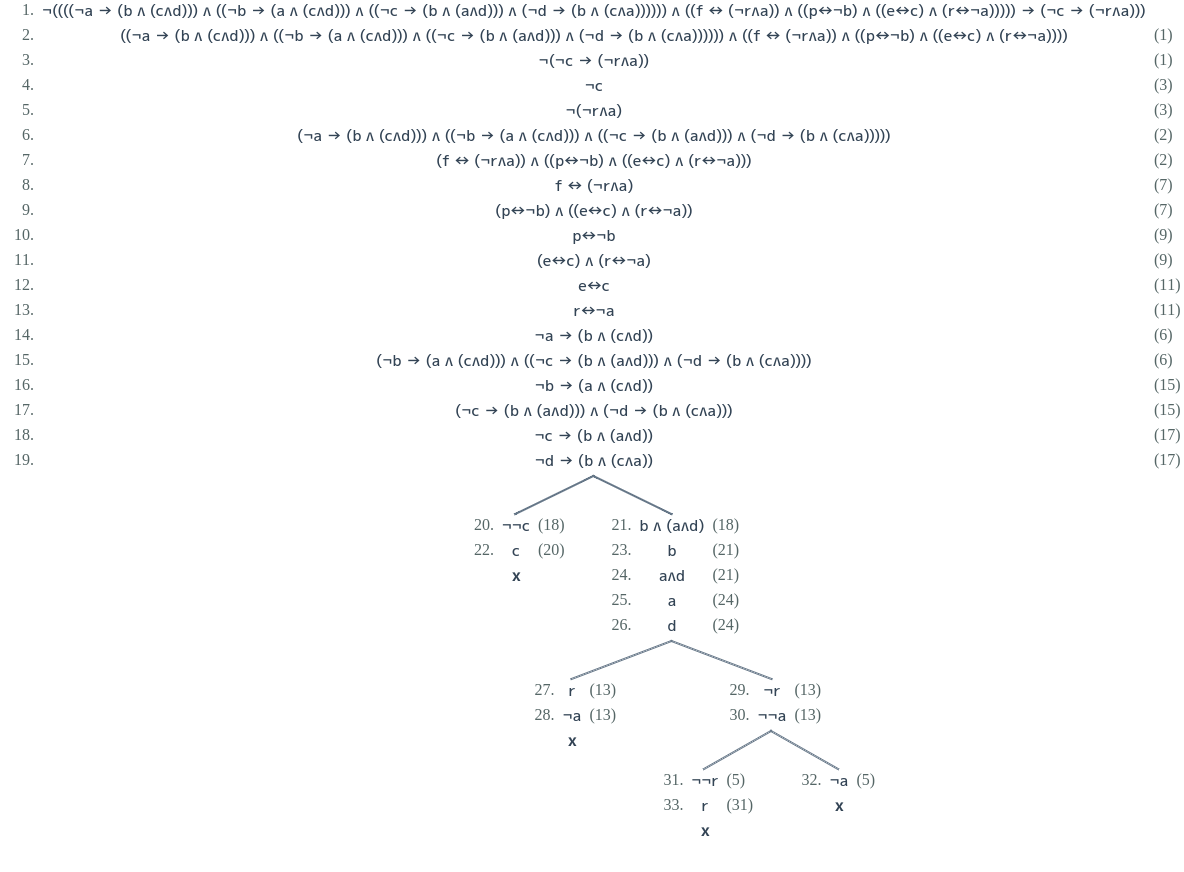
\includegraphics[scale=0.40]{img/problem2tableaux.png}
			\caption{ Demostracion por Tableaux}
			\label{fig:tableaux}
		\end{figure}

		
		\item Considere las siguientes informaciones:
		\begin{itemize}
		    \item Si el profesor tomara un examen, entonces los alumnos van bien o mal en el examen.
		    \item Si los alumnos fueren bien, entonces el profesor va a pensar que el examen estaba fácil y quedará frustrado.
		    \item Si los alumnos fueren mal, entonces el profesor va a pensar que los alumnos no aprendieron nada de lógica y quedará frustrado.
		\end{itemize}
		Queremos saber si podemos, a partir del texto, concluir que:
		\begin{enumerate}
		    \item Si el profesor tomara un examen, entonces el profesor quedará frustrado.
		    \item Si el profesor no tomara un examen, entonces el profesor no quedará frustrado.
		\end{enumerate}
		
		
		Declaración de las variables para formar las premisas: \\
		
		P. Profesor toma el examen\\
		F. Profesor frustrado\\
		A: Alumnos dan bien el examen\\
		L: Alumnos aprenden logica\\
		E: Examen facil\\
		\[ P \to (A \lor \neg A), A \to (E \land F), \neg A \to (\neg L \land F ) \]
		\[ Conclusiones \]
		\[ P \to F \]
		\[ \neg P \to \neg F \]
		   
                \[ Tableux \]
		        \[ P \to (A \lor \neg A), A \to (E \land F), \neg A \to (\neg L \land F ) \models P \to F \]
		        \begin{figure}[H]
        			\centering
        			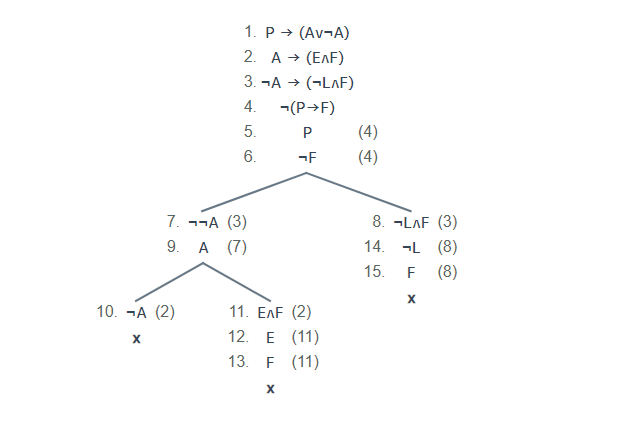
\includegraphics[scale=0.80]{img/ejercicio_03.png}
        			\caption{Demostración Tableaux, llegando a la conclusión que \textbf{ el profesor toma el examen entoces el profesor quedará frustrado}}
        			\label{fig:3_1}
        		\end{figure}
            

		
		\item Muestre que el conjunto de conectivos $\{\neg,\lor\}$ es completo. O sea, presente fórmulas $\varphi$ y $\psi$ conteniendo apenas los conectivos `$\neg$' y `$\lor$' tales que $\varphi \equiv \alpha \land \beta$ y $\psi \equiv \alpha \to \beta$. Justifique su respuesta usando tableaux.
		
		 \[ Conectivos \thinspace \{\neg \ , \lor \} \quad \quad \quad \quad \phi , \psi \thinspace deben \thinspace contener \]
		        \[ \varphi \equiv \alpha \land \beta  \qquad \qquad \qquad  \psi \equiv \alpha \to \beta \]
		        \[ \varphi \equiv \neg ( \neg \alpha \lor \neg \beta )  \qquad \qquad \psi \equiv \neg \alpha \lor \beta  \]
		          \[ \]
		        \[ Tableaux \]
		        \[ \neg ( \neg \alpha \lor \neg \beta ) \leftrightarrow \alpha \land \beta 
		        \qquad  \qquad  \qquad  \qquad  \qquad  \qquad 
		         \neg \alpha \lor \beta \leftrightarrow \alpha \to \beta \]
		         
		         \begin{figure}[H]
        			\centering
        			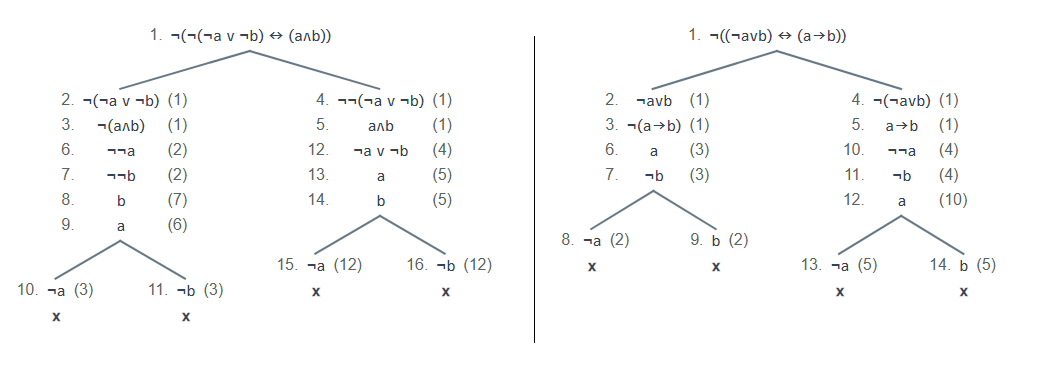
\includegraphics[scale=0.60]{img/ejercicio_04.png}
        			\caption{Demostración Tableaux con los cambios de los conectores `$\neg$' y `$\lor$' \textbf{si cierran}, por lo tanto \textbf{si son válidos}}
        			\label{fig:4_1}
        		\end{figure}
		
		\item Sea `$|$' (léase ``nand") un conectivo binario tal que $\alpha | \beta \equiv \neg(\alpha \land \beta)$. Muestre que el conjunto $\{|\}$ conteniendo apenas ese conectivo es completo. O sea, presente fórmulas $\varphi_1, \varphi_2, \varphi_3, \varphi_4$ conteniendo apenas el conectivo `$|$' tales que $\varphi_1 \equiv \neg\alpha, \varphi_2 \equiv \alpha\land\beta, \varphi_3 \equiv \alpha\lor\beta$ y $\varphi_4 \equiv \alpha \to \beta$. Justifique su respuesta usando tableaux.
		
		\begin{enumerate}
		    %%% primera formula
		    \item $\varphi_1 \equiv \neg\alpha,$ para completar la forma del conectivo nand, se utiliza la ley de idempotencia para que pueda aplicarse sobre la fórmula, $\alpha \land \alpha \equiv \alpha$, luego negando $\neg(\alpha \land \alpha) \equiv \neg(\alpha)$, quedando de la siguiente forma , ver figura \ref{fig:5_1}
		    \begin{equation}
		        \varphi_1 \equiv \alpha | \alpha \equiv \neg (\alpha \land \alpha)
		    \end{equation}
		    
		    \begin{figure}[H]
    			\centering
    			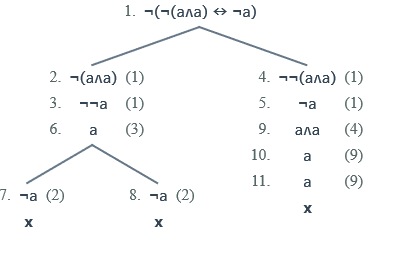
\includegraphics[scale=0.40]{img/5_1.png}
    			\caption{Demostrando por Tableaux la premisa $\varphi_1 \equiv \neg\alpha$}
    			\label{fig:5_1}
    		\end{figure}\
    		
    		%% segunda formula
    		\item $\varphi_2 \equiv \alpha\land\beta$, en este caso se interpreta recursivamente a ambas variables, $\alpha$ y $\beta$, para igualar a la formula de nand, la primera forma obedece a la negación de la conjunción ($\neg(\alpha \land \beta)$) y la segunda de la misma manera, para continuar con la recursión se aplica hacia arriba.
    		
    		\begin{equation}
		        \varphi_2 \equiv (\alpha | \beta) | (\alpha | \beta) \equiv \neg ( \neg (\alpha \land \beta) \land \neg  (\alpha \land \beta)) 
		    \end{equation}
		    
		    \begin{figure}[H]
    			\centering
    			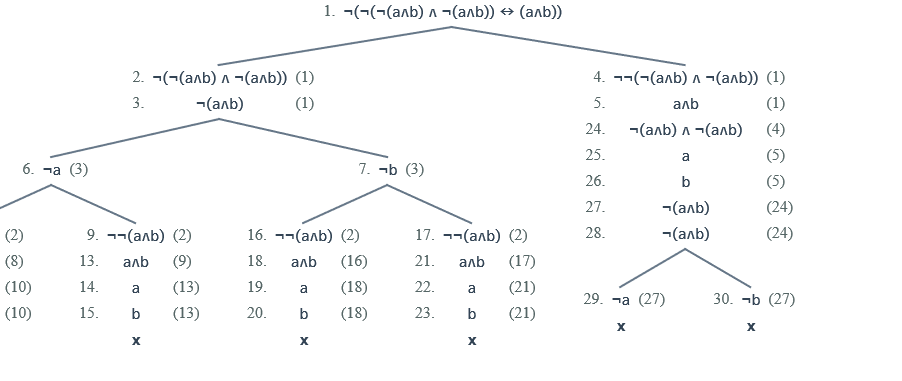
\includegraphics[scale=0.40]{img/5_2.png}
    			\caption{Demostrando por Tableaux la premisa $\varphi_2 \equiv \alpha\land\beta$}
    			\label{fig:5_2}
    		\end{figure}
    		
    		%%% tercera formula
    		\item $\varphi_3 \equiv \alpha\lor\beta$, para el caso de la disyunción aplicando la propiedad de equivalencia a la conjunción se aplica lo siguiente $\alpha \lor \beta \equiv \neg(  \neg \alpha \land \neg \beta)$ e igualmente realizando recursivamente la resolución de llamada al operador nand, empezando por resolver la negación tanto en $\alpha$ como en $\beta$ y siguiendo con la conjunción al finalizar, ver figura \ref{fig:5_3}.
    		
    		\begin{equation}
		        \varphi_3 \equiv (\alpha | \alpha) | (\beta | \beta) \equiv \neg ( \neg (\alpha \land \alpha) \land \neg ( \beta \land \beta)) 
		    \end{equation}
		    
		    \begin{figure}[H]
    			\centering
    			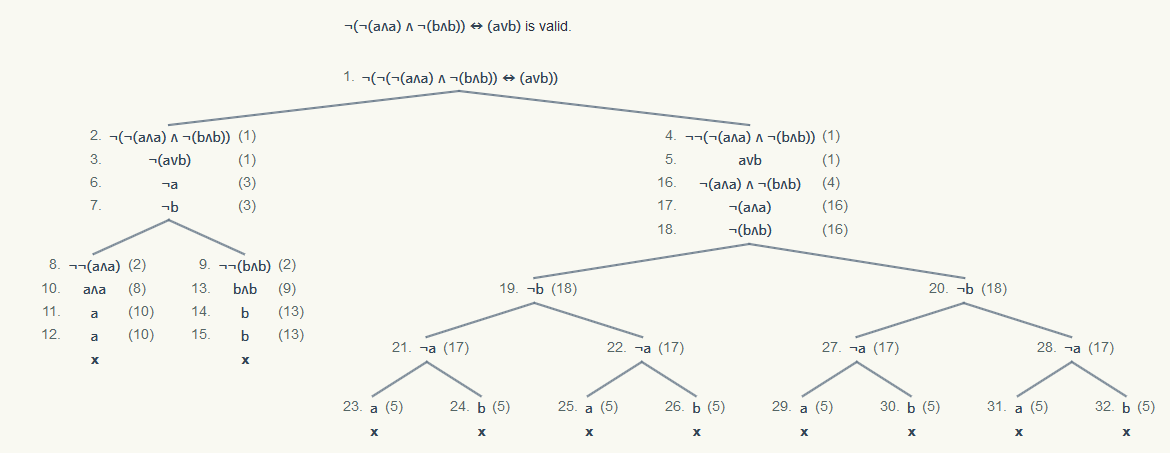
\includegraphics[scale=0.48]{img/5_3.png}
    			\caption{Demostrando por Tableaux la premisa $\varphi_3 \equiv \alpha\lor\beta$}
    			\label{fig:5_3}
    		\end{figure}
    		
    		%%% cuarta formula
    		
    		\item $\varphi4_ \equiv \alpha \to \beta$, previamente para la resolución igualemente aplicando la equivalencia con la disyunción se aplica $\alpha \to \beta \equiv \neg \alpha \lor \beta$ luego al igual que en $\varphi_3$ se aplica la equivalencia de la conjunción sin aun aplicar la ley de doble negación para continuar con la resolución $\neg (\neg \alpha) \land \beta$, finalmente resolviendo por recursión se aplica hacia las variables negadas $\neg (\neg \alpha \land \neg \alpha) \land \neg (\beta \land \beta))$ finalmente la propiedad de idempotencia y recursión nuevamente. \\
    		$ \neg(\neg (\neg (\alpha \land \alpha) \land \neg (\alpha \land \alpha)) \land \neg (\beta \land \beta))$, quedando de la siguiente forma, ver figura \ref{fig:5_4}
    		
    		\begin{equation}
		        \varphi4 \equiv ((\alpha | \alpha) | (\alpha | \alpha)) | (\beta | \beta) \equiv \neg(\neg (\neg (\alpha \land \alpha) \land \neg (\alpha \land \alpha)) \land \neg (\beta \land \beta)) 
		    \end{equation}
    		
    		\begin{figure}[H]
    			\centering
    			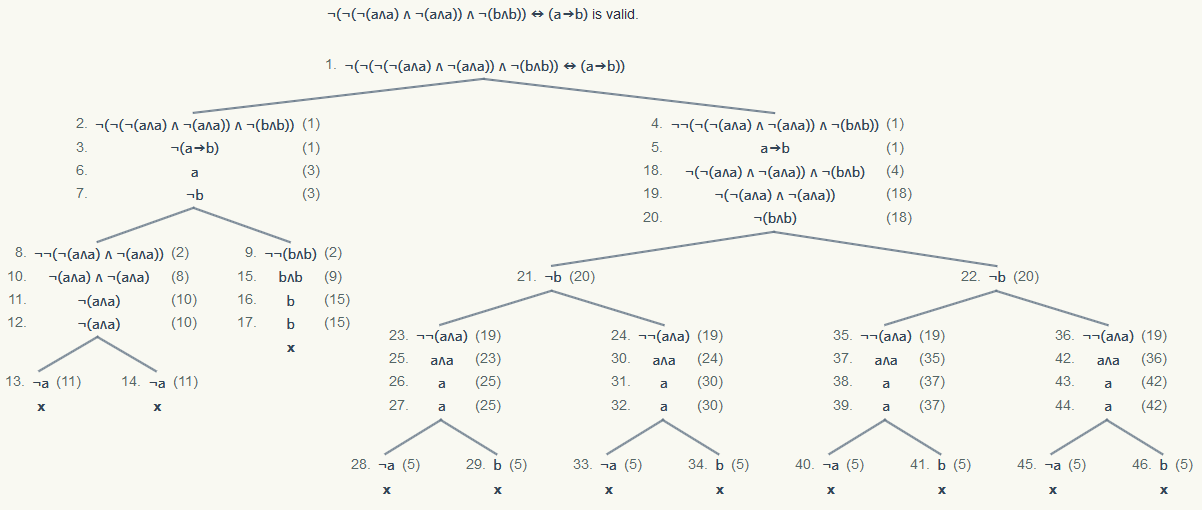
\includegraphics[scale=0.48]{img/5_4.png}
    			\caption{Demostrando por Tableaux la premisa $\varphi_4 \equiv \alpha \to \beta$}
    			\label{fig:5_4}
    		\end{figure}
		    
		\end{enumerate}
		
		\item Presente posibles reglas de Tableaux para el conectivo nand ($|$) del ejercicio anterior.
		    \begin{itemize}
		        \item Tomando la resolución de la operación $\alpha | \beta \equiv \neg(\alpha \land \beta)$ deberíamos tener en cuenta dos casos principales, primero la resolución de cuando es verdadera, ver figura \ref{fig:6_1}
		            \begin{figure}[H]
            			\centering
            			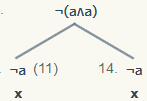
\includegraphics[scale=0.80]{img/6_1.png}
            			\caption{$V(\neg(\alpha \land \beta))$}
            			\label{fig:6_1}
            		\end{figure}
            	\item Y también de la resolución cuando es falsa, ver figura \ref{fig:6_2}
            	    \begin{figure}[H]
            			\centering
            			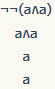
\includegraphics[scale=0.80]{img/6_2.PNG}
            			\caption{$F(\neg(\alpha \land \beta))$}
            			\label{fig:6_2}
            		\end{figure}
		    \end{itemize}
		    
		    Se puede concluir que:
		    
		    \begin{equation}
		        \frac{ V(\alpha | \beta)}{F(\alpha) |F(\beta)} \ \ \frac{F(\alpha | \beta)}{ \begin{matrix} V(\alpha)  \\  V(\beta) \end{matrix}}   
		    \end{equation}
		     

		
		
		
		\item Deduzca, por el método de Deducción Natural, si $\neg P \to Q$ es consecuencia lógica del conjunto de proposiciones: $\{ P \lor (Y \to X),X \to Z, (Y \to Z) \to Q \}$. Se uso como referencia para la deducción natural \cite{huth2004logic}, llegando a concluir y cerrando cada nueva premisa.
		    \begin{itemize}
    		     \item Proposiciones: 
    		     \begin{equation}
    		     \begin{aligned}
    		        P \vee (Y \rightarrow X)\\
    		        (X \rightarrow Z)\\
    		        ((Y \rightarrow Z) \rightarrow Q)
    		     \end{aligned}
    		     \end{equation}
    		 \end{itemize}
    		 
    		 \begin{prooftree}
    		    \AxiomC{$ [\neg P]^1$}
    		    \AxiomC{$ (P \vee (Y \rightarrow X))$}
                \RightLabel{Modus Tollendo Ponens}
    		    \BinaryInfC{$Y \rightarrow X$}
    		    \UnaryInfC{$[Y]^2$ $Y \rightarrow X$}
    		    \RightLabel{Modus Ponendo Ponens}
    		    \UnaryInfC{$X$ $(X \rightarrow Z)$}
    		    \RightLabel{Modus Ponendo Ponens}
    		    \UnaryInfC{$Z$}
    		    \UnaryInfC{$[Y]^2 \rightarrow Z$}
    		    \UnaryInfC{$[Y]^2 \rightarrow Z$ $((Y \rightarrow Z) \rightarrow Q)$}
    		    \RightLabel{Modus Ponendo Ponens}
    		    \UnaryInfC{$Q$}
    		    \UnaryInfC{$\neg P \rightarrow Q$}
    		 \end{prooftree}
		
		
		\item Pruebe la sentencia abajo usando Deducción Natural \\
		        $\{ A \lor (B \land C), \neg E, (A \lor B) \to (D \lor E)),\neg A \} \vdash (C \land D)$
		 
    		 \begin{itemize}
    		     \item Propiedad Distributiva: 
    		     \begin{equation}
    		     \begin{aligned}
    		     A \vee (B \wedge C) \equiv (A \vee B) \wedge (A \vee C)\\
    		     \end{aligned}
    		     \end{equation}
    		 \end{itemize}
    		 
    		 \begin{prooftree}
    		    \AxiomC{$A \vee (B \wedge C)$}
    		    \UnaryInfC{$ (A \vee B) \wedge (A \vee C)$}
    		    \UnaryInfC{$ (A \vee B) (A \vee B) \rightarrow (D \vee E)$}
    		    \LeftLabel{modus ponendo ponens}
    		    \UnaryInfC{$ (D \vee E) \neg E$}
    		    \UnaryInfC{$ \neg E (\neg D \rightarrow E)$}
    		    \UnaryInfC{$ \neg E (\neg E \rightarrow D)$}
    		    \LeftLabel{modus tollendo ponens}
    		    \UnaryInfC{$ D$}
    		    
    		    \AxiomC{$A \vee (B \wedge C)$}
    		    \UnaryInfC{$ (A \vee B) \wedge (A \vee C)$}
    		    \UnaryInfC{$ (A \vee C) \neg A$}
    		    \UnaryInfC{$ \neg A( \neg A \rightarrow C)$}
    		    \RightLabel{modus tollendo ponens}
    		    \UnaryInfC{$ C $}
    		    \RightLabel{$I \wedge$}
    		    \BinaryInfC{$C \wedge D$}
    		 \end{prooftree}
		    
		 
		 \item Considere lo siguiente: ``Si Beto pelea con Gloria, entonces Gloria va al cine. Si Gloria va a cine, entonces Carla se queda en casa. Si Carla se queda en casa, entonces Raúl pelea con Carla. Ahora, Raúl no pelea con Carla". Escriba un conjunto de fórmulas que describe el problema. Verifique cual de estas alternativas es consecuencia lógica de las fórmulas que especifican el problema. Use Deducción Natural para probar la consecuencia lógica.
		 \begin{enumerate}
		     \item Carla no se queda en casa y Beto no pelea con Gloria.
		     \item Carla se queda en casa y Gloria va al cine.
		     \item Carla no se queda en casa y Gloria va al cine.
		     \item Gloria va al cine y Beto pelea con Gloria.
		     \item Gloria no va al cine y Beto pelea con Gloria.
		 \end{enumerate}
		 
		 Solución \\
		\begin{itemize}
		    \item p: Beto pelea con Gloria.
		    \item q: Gloria va al cine.
		    \item r: Carla se queda en casa.
		    \item s: Raúl pelea con Carla.
		\end{itemize}
		
		 \begin{enumerate}
		 
		    \item Carla no se queda en casa y Beto no pelea con Gloria.
		        \begin{equation}
                    \{ p  \to q, q \to r, r \to s, \neg s
                    \} \models \neg r \land \neg p
                \end{equation}
                
                \begin{prooftree}
        		    \AxiomC{$r \rightarrow s$}
        		    \AxiomC{$\neg s$}
        		    \BinaryInfC{$  \neg r$}
        		    \RightLabel{Tollendo Tollens}
        		    \UnaryInfC{$ (q \rightarrow r) $ $ \neg r$}
        		    \RightLabel{Tollendo Tollens}
        		    \UnaryInfC{$ (p \rightarrow q) $ $ \neg q$}
        		    \RightLabel{Tollendo Tollens}
        		    \UnaryInfC{$\neg p$}
        		    \RightLabel{$I \wedge$}
        		    \UnaryInfC{$ \neg p$ $ \neg r$}
        		    \UnaryInfC{$\neg r \wedge \neg p$}
        		\end{prooftree}
                
		    \item Carla se queda en casa y Gloria va al cine.
		        \begin{equation}
                    \{ p  \to q, q \to r, r \to s, \neg s
                    \} \models  r \land q
                \end{equation}
                
               \begin{prooftree}
        		    \AxiomC{$r \rightarrow s$}
        		    \AxiomC{$\neg s$}
        		    \BinaryInfC{$  \neg r$}
        		    
        		    \AxiomC{$q \rightarrow r$}
        		    \AxiomC{$\neg r$}
        		    \BinaryInfC{$  \neg q$}
        		    \BinaryInfC{$ \neg r$ $\neg q$ $ \vdash \neg r \wedge \neg q$}
        		    \RightLabel {Contradiccion en $r$ y $q$}
        		    \UnaryInfC{$r$ $q$ $\vdash r \wedge q$}
        		    
        		\end{prooftree}
                
		    \item Carla no se queda en casa y Gloria va al cine.
		        \begin{equation}
                    \{ p  \to q, q \to r, r \to s, \neg s
                    \} \models \neg r \land q
                \end{equation}
                
                \begin{prooftree}
        		    \AxiomC{$r \rightarrow s$}
        		    \AxiomC{$\neg s$}
        		    \BinaryInfC{$  \neg r$}
        		    
        		    \AxiomC{$q \rightarrow r$}
        		    \AxiomC{$\neg r$}
        		    \BinaryInfC{$  \neg q$}
        		    \BinaryInfC{$ \neg r$ $\neg q$ $ \vdash \neg r \wedge \neg q$}
        		    \RightLabel {Contradiccion en $q$}
        		    \UnaryInfC{$\neg r$ $q$ $\vdash \neg r \wedge q$}
        		\end{prooftree}
		    \item Gloria va al cine y Beto pelea con Gloria.
		        \begin{equation}
                    \{  p  \to q, q \to r, r \to s, \neg s
                    \} \models q \land p
                \end{equation}
                \begin{prooftree}
        		    \AxiomC{$[p]^1$}
        		    \AxiomC{$ p \to q$}
        		    \RightLabel{Modus Ponendo Ponens}
        		    \BinaryInfC{$q$ $ q \to r$}
        		    \RightLabel{Modus Ponendo Ponens}
        		    \UnaryInfC{$ r $ $ r \to s$}
        		    \RightLabel{Modus Ponendo Ponens}
        		    \UnaryInfC{$s$ $ \neg s$}
        		    \RightLabel{$I \land $}
        		    \UnaryInfC{$\bot$ $r$}
        		    \RightLabel{Absurdo}
        		    \UnaryInfC{$\neg r $ }
        		    \UnaryInfC{$ q \land [p]^1 $ }
        		\end{prooftree}
		    \item Gloria no va al cine y Beto pelea con Gloria.
		        \begin{equation}
                    \{ p  \to q, q \to r, r \to s, \neg s
                    \} \models \neg q \land  p
                \end{equation}
                \begin{prooftree}
        		    \AxiomC{$[p]^1$}
        		    \AxiomC{$ p \to q$}
        		    \RightLabel{Modus Ponendo Ponens}
        		    \BinaryInfC{$q$ $ q \to r$}
        		    \RightLabel{Modus Ponendo Ponens}
        		    \UnaryInfC{$ r $ $ r \to s$}
        		    \RightLabel{Modus Ponendo Ponens}
        		    \UnaryInfC{$s$ $ \neg s$}
        		    \RightLabel{$I \land $}
        		    \UnaryInfC{$\bot$ $q$}
        		    \RightLabel{Absurdo}
        		    \UnaryInfC{$\neg q $ $\land $ $[p]^1$}
        		    \RightLabel{$I \land $}
        		\end{prooftree}
		    \end{enumerate}
		    
		    Concluyendo que solamente en \textbf{ $(a)$ Carla no se queda en casa y Beto no pelea con Gloria}, concluye y finaliza las premisas.
		
	\end{enumerate}


	
	\clearpage
	%\bibliographystyle{apalike}
	\bibliographystyle{IEEEtranN}
	\bibliography{bibliography}
		
	
\end{document}